\documentclass{beamer} %[aspectratio=1610]

\usetheme{Darmstadt}
\usefonttheme[onlylarge]{structurebold}
\setbeamerfont*{frametitle}{size=\normalsize,series=\bfseries}
\setbeamertemplate{navigation symbols}{}

% Standard packages

\usepackage[english]{babel}
\usepackage[latin1]{inputenc}
\usepackage{times}
\usepackage[T1]{fontenc}
\usepackage{float}
\usepackage{graphicx}
\usepackage{subcaption}
\usepackage{ifthen}
\usepackage{minted}
\usepackage{verbatim}
%\usepackage{multimedia}
\usepackage{movie15}

% Setup TikZ
\usepackage{tikz}
\usetikzlibrary{arrows}
\tikzstyle{block}=[draw opacity=0.7,line width=1.4cm]


% Author, Title, etc.
\title[Pure functional programming in Agent-Based Simulation] 
{%
  Pure functional programming \\ in Agent-Based Simulation
}

\author[Thaler]
{
  Jonathan~Thaler
}

\institute[University of Nottingham, Ningbo, China]
{
  University of Nottingham, Ningbo, China
}

\date[AIOP Seminar 2019]
{AIOP Seminar 2019}

% The main document
\begin{document}

\begin{frame}
  \titlepage
\end{frame}

\section{Introduction}
\begin{frame}{The Metaphor}
\begin{itemize}
  \item "[..] object-oriented programming is a particularly natural development environment for Sugarscape specifically and artificial societies generally [..]" (Epstein et al 1996)
  
  \item "agents map naturally to objects" (North et al 2007)
\end{itemize}
\end{frame}

\begin{frame}{Outline}
\begin{itemize}
  \item What is Agent-Based Simulation (ABS)?
  
  \item What is \textit{pure} Functional Programming (FP)?
  
  \item How can we do ABS + FP?  
  
  \item ABS + FP = ?
  
  \item Conclusions
\end{itemize}
\end{frame}

\section{Agent-Based Simulation}
\begin{frame}{What is Agent-Based Simulation (ABS)?} 
  \begin{block}{Example}
    \textit{\textbf{Simulate} the spread of an infectious disease in a city. \\ What are the \textbf{dynamics} (peak, duration of disease)?}
  \end{block}
  
  \begin{enumerate}
    \item Start with population \, \, \, \, \, \, \, $\to$ Agents
 	\item Situated in City \, \, \, \, \, \, \, \, \, \, \, \,\, $\to$ Environment
 	\item Interacting with each other \, $\to$ Local interactions
 	\item Creating dynamics \, \, \, \, \, \, \, \,\,\, $\to$ Emergent system behaviour
 	\item Therefore ABS \, \, \, \, \, \, \, \, \, \, \, \,\,\, $\to$ Bottom-up approach
  \end{enumerate}
\end{frame}

\begin{frame}{SIR Model}
  
\includegraphics[width=0.7\textwidth]{./fig/SIR_transitions.png}
  
  \begin{itemize}
    \item Population size $N = 1,000$
 	\item Contact rate $\beta = 5$
 	\item Infection probability $\gamma = 0.05$
 	\item Illness duration $\delta = 15$
 	\item 1 initially infected agent
  \end{itemize}
    
  \begin{block}{System Dynamics}
    Top-Down, formalised using Differential Equations, give rise to dynamics.
  \end{block}
\end{frame}

\begin{frame}{SIR Model Dynamics}
  \center
  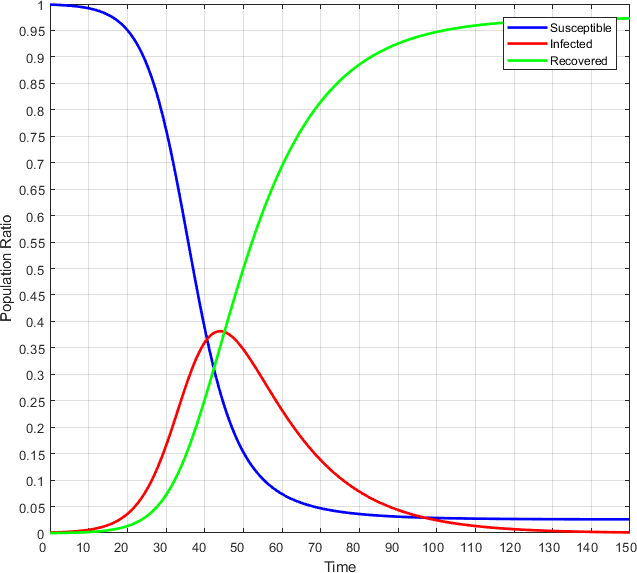
\includegraphics[width=0.7\textwidth]{./fig/SIR_SD_001dt.png}
\end{frame}

\begin{frame}[fragile]{Defining Spatiality}
\begin{figure}
\begin{center}

\includegraphics[width=0.2\textwidth]{./fig/moore.png}
\caption*{Moore Neighbourhood}
\end{center}
\end{figure}
\end{frame}

\begin{frame}{Spatial Dynamics}
\begin{figure}
\begin{center}
	\begin{tabular}{c c}
		\begin{subfigure}[b]{0.4\textwidth}
			\centering
			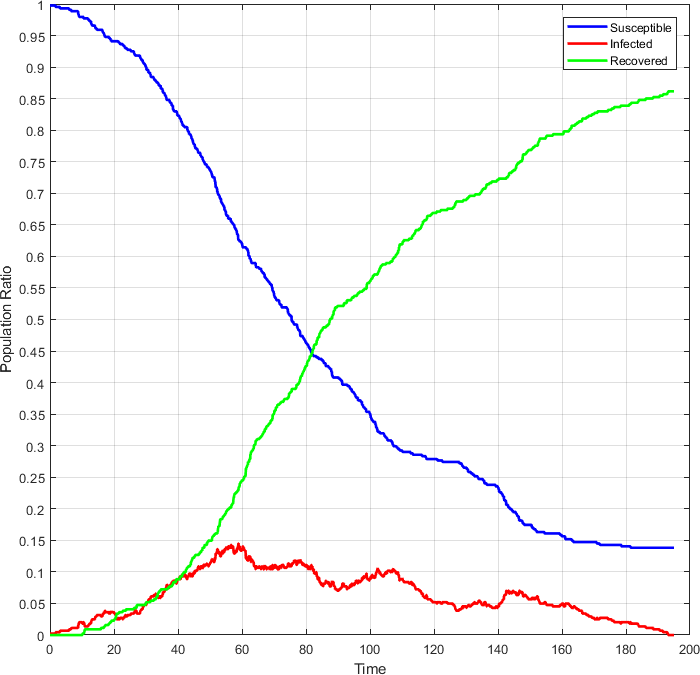
\includegraphics[width=0.95\textwidth, angle=0]{./fig/SIR_Dunai_dt001.png}
			\caption*{Agent-Based}
		\end{subfigure}
    	
    	&
  
		\begin{subfigure}[b]{0.4\textwidth}
			\centering
			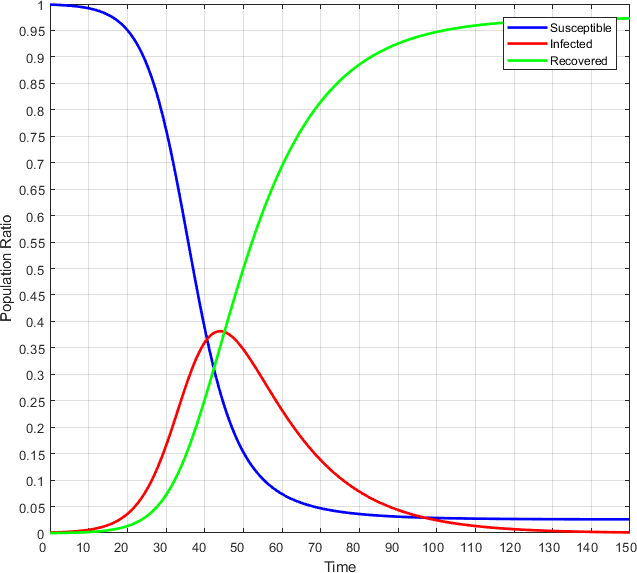
\includegraphics[width=1\textwidth, angle=0]{./fig/SIR_SD_001dt.png}
			\caption*{System Dynamics}
		\end{subfigure}
	\end{tabular}
\end{center}
\end{figure}
\end{frame}

\begin{frame}{Spatial Visualisation}
%\movie[width=10cm,height=5.5cm]{Dynamics 21x21 2D Environment}{./video/SIR_DUNAI_dt001.mp4}
\includemovie[rate=2]{11cm}{6.5cm}{./video/SIR_DUNAI_dt001.mp4}
\end{frame}

\section{Pure functional programming}
\begin{frame}[fragile]{What is pure functional programming?}
  \begin{block}{Functions as first class citizens}
  	Passed as arguments, returned as values and assigned to variables.
  \end{block}
  
  \begin{block}{}
  \begin{minted}[fontsize=\normalsize]{haskell}
  map :: (a -> b) -> [a] -> [b]
	
  const :: a -> (b -> a)
  const a = (\_ -> a)
  \end{minted}
  \end{block}
\end{frame}
 
\begin{frame}[fragile]{What is pure functional programming cont'd?}
  \begin{block}{Immutable data}
 	Variables can not change, functions return new copy. \\ Data-Flow oriented programming.
  \end{block}
  
  \begin{block}{}
  \begin{minted}[fontsize=\normalsize]{haskell}
  let x   = [1..10]
      x'  = drop 5 x
      x'' = x' ++ [10..20] 
  \end{minted}
  \end{block}
\end{frame}
 
\begin{frame}[fragile]{What is pure functional programming cont'd?}
  \begin{block}{Recursion}
 	To iterate over and change data. 
  \end{block}
  
  \begin{block}{}
  \begin{minted}[fontsize=\normalsize]{haskell}
  fact :: Int -> Int
  fact 0 = 1
  fact n = n * fact (n-1)
  \end{minted}
  \end{block}
\end{frame}
 
\begin{frame}[fragile]{What is pure functional programming cont'd?}
  \begin{block}{Declarative style}
  	Describe \textit{what} to compute instead of \textit{how}.
  \end{block}
  
  \begin{block}{}
  \begin{minted}[fontsize=\normalsize]{haskell}
  mean :: [Double] -> Double
  mean xs = sum xs / length xs
  \end{minted}
  \end{block}
\end{frame}
 
\begin{frame}[fragile]{What is pure functional programming cont'd?}
  \begin{block}{Explicit about Side-Effects}
  	Distinguish between side-effects of a function \textit{in its type}.
  \end{block}
  
  \begin{block}{}
  \begin{minted}[fontsize=\normalsize]{haskell}
  readFromFile      :: String -> IO String
  randomExponential :: Double -> Rand Double
  statefulAlgorithm :: State Int (Maybe Double)
  produceData       :: Writer [Double] ()
  \end{minted}
  \end{block}
\end{frame}

\section{ABS + FP}
\begin{frame}{How can we do ABS + FP?}
  \begin{block}{How can we represent an Agent, its local state and its interface?}
	We don't have objects and mutable state...
  \end{block}
  
  \begin{block}{How can we implement direct agent-to-agent interactions?}
	We don't have method calls and mutable state...
  \end{block}
  
  \begin{block}{How can we implement an environment and agent-to-environment interactions?}
	We don't have method calls and mutable state...
  \end{block}
  
  \begin{block}{Solution}
  	Functional Reactive Programming + \\ Monadic Stream Functions
  \end{block}
\end{frame}

\begin{frame}{Arrowized Functional Reactive Programming (AFRP)}
  \begin{itemize}
    \item Continuous- \& discrete-time systems in FP
 	\item Signal Function 
 	\item Events
 	\item Effects like random-numbers, global state, concurrency
 	\item \textit{Arrowized} FRP using the \textit{Dunai} library
  \end{itemize}
\end{frame}

\begin{frame}{Monadic Stream Functions (MSF)}
  \begin{block}{Process over time}
  \begin{flalign*}
	SF \, \alpha \, \beta \approx Signal \, \alpha \rightarrow Signal \, \beta \\
	Signal \, \alpha \approx Time \rightarrow \alpha 
  \end{flalign*}
  \end{block}
  
  \begin{block}{Agents as Signal Functions}
  \begin{itemize}
  	\item Clean interface (input / output)
  	\item Pro-activity by perceiving time
  	\item Closures + Continuations = very simple immutable objects
  \end{itemize}
  \end{block}
\end{frame}

\begin{frame}[fragile]{What are closures and continuations?}
\begin{block}{}
\begin{minted}[fontsize=\footnotesize]{haskell}
-- continuation type-definition
newtype Cont a = Cont (a -> (a, Cont a))

-- A continuation which sums up inputs.
-- It uses a closure to capture the input
adder :: Int -> Cont Int
adder x = Cont (\x' -> (x + x', adder (x + x')))
\end{minted}
\end{block}
\end{frame}

%-- Runs a continuation for n steps and
%-- prints the output in each step
%runCont :: Int -> Cont Int -> IO ()
%runCont 0 _ = return ()
%runCont n (Cont cont) = do
%  let (x, cont') = cont 1
%  print x
%  runCont (n-1) cont'

\begin{frame}[fragile]{Recovered Agent}
\begin{block}{}
\begin{minted}[fontsize=\footnotesize]{haskell}
data SIRState    = Susceptible | Infected | Recovered

type Disc2dCoord = (Int, Int)
type SIREnv      = Array Disc2dCoord SIRState

type SIRAgent    = SF Rand SIREnv SIRState

recoveredAgent :: SIRAgent
recoveredAgent = arr (const Recovered) 
\end{minted}
\end{block}
\end{frame}

\begin{frame}[fragile]{Infected Agent}
\begin{block}{}
\begin{minted}[fontsize=\footnotesize]{haskell}
infectedAgent :: Double -> SIRAgent
infectedAgent delta
    = switch infected (const recoveredAgent)
  where
    infected :: SF Rand SIREnv (SIRState, Event ())
    infected = proc _ -> do
      recovered <- occasionally delta () -< ()
      if isEvent recovered
        then returnA -< (Recovered, Event ())
        else returnA -< (Infected, NoEvent)
\end{minted}
\end{block}
\end{frame}

\begin{frame}[fragile]{Susceptible Agent}
\begin{block}{}
\begin{minted}[fontsize=\footnotesize]{haskell}
susceptibleAgent coord beta gamma delta 
    = switch susceptible (const (infectedAgent delta))
  where
    susceptible :: SF Rand SIREnv (SIRState, Event ())
    susceptible = proc env -> do
      makeContact <- occasionally (1 / beta) () -< ()
      if isEvent makeContact
        then (do
          s <- randomNeighbour coord env -< as
          case s of
            Just Infected -> do
              i <- arrM_ (lift (randomBoolM gamma)) -< ()
              if i
                then returnA -< (Infected, Event ())
                else returnA -< (Susceptible, NoEvent)
            _       -> returnA -< (Susceptible, NoEvent))
        else returnA -< (Susceptible, NoEvent)
\end{minted}
\end{block}
\end{frame}

\section{ABS + FP = ?}
\begin{frame}{ABS + FP = Type Saftey}
	\begin{block}{Purity guarantees reproducibility at compile time}
    "... when the sequence of random numbers is specified ex ante the model is deterministic. Stated yet another way, model output is invariant from run to run when all aspects of the model are kept constant including the stream of random numbers." Epstein et al (1996)
    \end{block}
\end{frame}

\begin{frame}{ABS + FP = Enforce Update Semantics}
  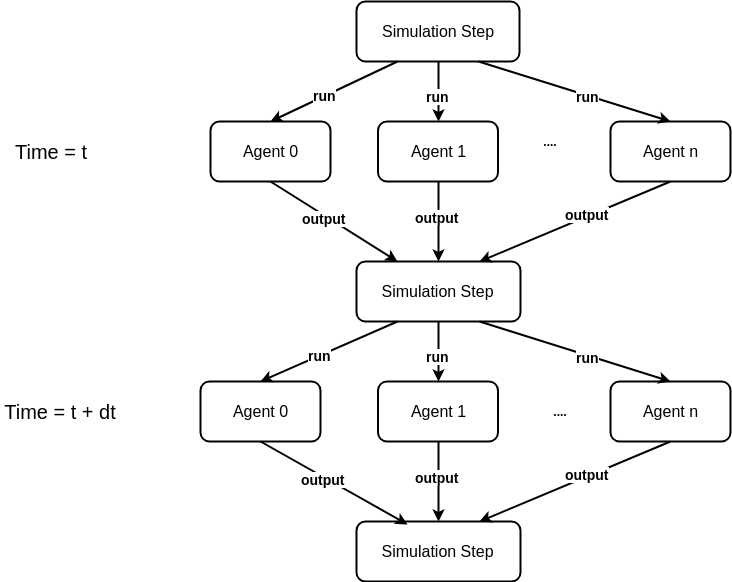
\includegraphics[width=0.7\textwidth]{./fig/parallel_strategy.png}
\end{frame}

\begin{frame}{ABS + FP = Software Transactional Memory}
  \begin{itemize}
  	\item Concurrency in ABS difficult.
	\item Synchronisation using locks.
  	\item $\Rightarrow$ error prone 
  	\item $\Rightarrow$ mixing of concurrency and model related code.
  	\item New approach in Haskell: Software Transactional Memory.
  \end{itemize}
\end{frame}

\begin{frame}{Software Transactional Memory (STM)}
  \begin{itemize}   	
  	\item Lock free concurrency.
  	\item Run STM actions concurrently and rollback / retry.
  	\item Haskell first language to implement in core.    
    \item Haskell type system guarantees retry-semantics.
  \end{itemize}
\end{frame}

\begin{frame}{Software Transactional Memory (STM)}
  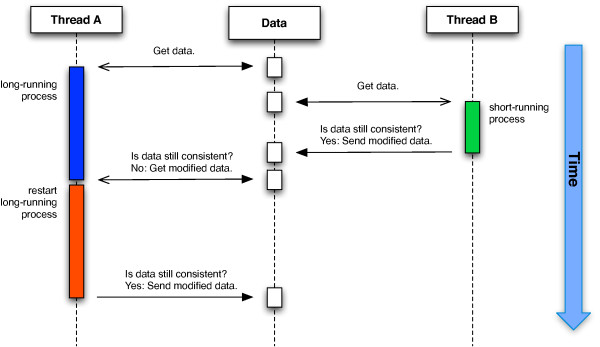
\includegraphics[width=0.9\textwidth]{./fig/stm.png}
\end{frame}

\begin{frame}{Software Transactional Memory (STM)}
  \begin{itemize}
  	\item Tremendous performance improvement.
    \item Substantially outperforms lock-based implementation.
    \item STM semantics retain guarantees about non-determinism.
  \end{itemize}
\end{frame}

\begin{frame}{ABS + FP = Property-Based Testing}
  \begin{itemize}
    \item Express specifications directly in code.
    \item QuickCheck library generates random test-cases.
    \item Developer can express expected coverage.
    \item Random Property-Based Testing + Stochastic ABS = $\heartsuit \heartsuit \heartsuit$
  \end{itemize}
\end{frame}

\begin{frame}[fragile]{QuickCheck}
\begin{block}{List Properties}
\begin{minted}[fontsize=\footnotesize]{haskell}
-- the reverse of a reversed list is the original list
reverse_reverse :: [Int] -> Bool
reverse_reverse xs 
  = reverse (reverse xs) == xs

-- concatenation operator (++) is associative
append_associative :: [Int] -> [Int] -> [Int] -> Bool
append_associative xs ys zs 
  = (xs ++ ys) ++ zs == xs ++ (ys ++ zs)

-- reverse is distributive over concatenation (++)
reverse_distributive :: [Int] -> [Int] -> Bool
reverse_distributive xs ys 
  = reverse (xs ++ ys) == reverse xs ++ reverse ys
\end{minted}
\end{block}
\end{frame}

\begin{frame}[fragile]{QuickCheck cont'd}
\begin{block}{Running the tests...}
\begin{footnotesize}
\begin{verbatim}
+++ OK, passed 100 tests.
+++ OK, passed 100 tests.
*** Failed! Falsifiable (after 3 tests and 1 shrink):     
[1]
[0]
\end{verbatim}
\end{footnotesize}
\end{block}
\end{frame}

\begin{frame}[fragile]{QuickCheck cont'd}
\begin{block}{Labeling}
\begin{minted}[fontsize=\footnotesize]{haskell}
reverse_reverse_label :: [Int] -> Property
reverse_reverse_label xs  
  = label ("length of list is " ++ show (length xs)) 
          (reverse (reverse xs) == xs)
\end{minted}
\end{block}

\begin{block}{Running the tests...}
\begin{footnotesize}
\begin{verbatim}
+++ OK, passed 100 tests:
 5% length of list is 27
 5% length of list is 15
 5% length of list is 0
 4% length of list is 4
 4% length of list is 19
 ...
\end{verbatim}
\end{footnotesize}
\end{block}
\end{frame}

\begin{frame}[fragile]{QuickCheck cont'd}
\begin{block}{Coverage}
\begin{minted}[fontsize=\footnotesize]{haskell}
reverse_reverse_cover :: [Int] -> Property
reverse_reverse_cover xs  = checkCoverage 
  cover 15 (length xs >= 50) "length of list at least 50"
  (reverse (reverse xs) == xs)
\end{minted}
\end{block}

\begin{block}{Running the tests...}
\begin{footnotesize}
\begin{verbatim}
+++ OK, passed 12800 tests 
    (15.445% length of list at least 50).
\end{verbatim}
\end{footnotesize}
\end{block}
\end{frame}

\begin{frame}{Property-Based Testing Conclusion}
  \begin{itemize}
    \item Test agent specification.
    \item Test simulation invariants.
    \item Validate dynamics against real world data.
    \item Exploratory models: hypotheses tests about dynamics.
    \item Explanatory models: validate against formal specification.
  \end{itemize}
\end{frame}

\section{Conclusion}
\begin{frame}{Conclusion}
\begin{block}{Have we done ABS implementation wrong?}
No, but we missed out on a lot of potential!
\end{block}
%
%  \begin{itemize} 
%  	\item First steps
%  	\item Develop library
%  	\item Performance
%    \item Goal is correct-by-construction implementation %The direction is towards an simulation which is more likely to be correct with the ultimate goal being a correct-by-construction implementation (up to some specification).
%    %\item A correct-by-construction implementation does NOT relief us from actually running the simulation!
%  \end{itemize}
\end{frame}

\begin{frame}{}
  \begin{center}
  Thank You!
  \end{center}
\end{frame}
\end{document}